\documentclass[sigconf,nonacm]{acmart}
\settopmatter{printacmref=false,printccs=false,printfolios=false}
\renewcommand\footnotetextcopyrightpermission[1]{}
\pagestyle{empty}
\raggedbottom
\newcommand{\ExperimentPlatform}{Talapas, Slurm job 48205110 on n0187}
\newcommand{\ExperimentCPU}{AMD EPYC 7713 64-Core Processor}
\newcommand{\ExperimentCompiler}{GCC 8.5.0}
\newcommand{\RunStatus}{Measured on the compute node inside the recorded Slurm allocation. Allocation: 64 CPUs and 4 GiB RAM.}
\newcommand{\MaxSize}{33,554,432}
\newcommand{\TrialCount}{7}
\newcommand{\ConfigurationCount}{60}
\newcommand{\MeasurementCount}{420}
\newcommand{\ThreadCounts}{1, 2, 4, 8, 16, 32, 64}
\newcommand{\SerialTime}{15.61}
\newcommand{\TreeTime}{18.34}
\newcommand{\TreeSpeedup}{0.85}
\newcommand{\TreeThreads}{64}
\newcommand{\DoublingTime}{98.12}
\newcommand{\DoublingSpeedup}{0.16}
\newcommand{\DoublingThreads}{64}
\newcommand{\ProblemSizes}{2^{16}, 2^{20}, 2^{24}, 2^{25}}
\newcommand{\HighThreadFinding}{At 64 threads, tree and doubling speedups were 0.85 and 0.16, respectively.}
\newcommand{\FindingSummary}{Neither parallel method's median time beat serial at any tested input size. Lower total work alone did not guarantee proportional thread scaling.}
\newcommand{\MachineLimit}{The node has 128 physical cores across two sockets and eight NUMA domains. The shared first-touch policy and core binding can affect serial/parallel ratios; this experiment does not isolate placement effects or characterize other nodes.}

\title{Parallel Prefix Sums: Work Efficiency and Thread Scaling}
\author{CIS 431/531 --- Homework 02}
\date{}
\begin{document}
\maketitle
\thispagestyle{empty}

\section{Algorithms}
For input $x$, all implementations compute the inclusive sum
$y_i=\sum_{j=0}^{i}x_j$ using the starter's 32-bit \texttt{int} data. The serial recurrence takes
$n-1$ additions. The first parallel implementation doubles its offset
$d=1,2,4,\ldots$: each level reads the previous buffer and writes
$y_i=x_i+x_{i-d}$ where the predecessor exists. Separate buffers and a
barrier between levels avoid read/write races. Its work is $O(n\log n)$
and span $O(\log n)$.

The second implementation uses the lecture's inclusive binary-tree
up-sweep/down-sweep. Upward stages form subtree sums; downward stages
propagate accumulated prefixes to the remaining positions. For
$n=2^k$, it performs $(n-1)+(n-1-k)$ additions: $O(n)$ work with
$O(\log n)$ span. Non-power-of-two lengths skip nonexistent positions.
Both parallel implementations keep one OpenMP team across all stages.

\section{Experimental method}
\textbf{Platform:} \ExperimentPlatform{}; \ExperimentCPU{};
\ExperimentCompiler{} with \texttt{-O3 -std=c99 -fopenmp}
(C++17 measurement driver).
\textbf{Execution status:} \RunStatus{}

We tested $n=\ProblemSizes$ with \ThreadCounts{} threads.
Inputs $x_i=(i\bmod201)-100$ keep intermediate sums in range.
Each configuration received one excluded warmup and \TrialCount{}
measured trials, shuffled in a reproducible order: \MeasurementCount{}
measurements across \ConfigurationCount{} configurations.
Monotonic wall-clock timings are used. The figure shows
median speedup and the interquartile range of runtimes transformed to
speedup using the serial median. Memory allocation, input generation,
validation, and CSV output are excluded; algorithm-internal copies, synchronization,
team overhead, and any final buffer copy are included. All arrays use
the same parallel first-touch policy. Threads are bound with
\texttt{OMP\_PLACES=cores} and \texttt{OMP\_PROC\_BIND=close}.
Every measured output is checked against the serial result outside
the timed region. Independent \texttt{std::partial\_sum} correctness
tests cover signed/zero/large values, empty input, and irregular lengths.
As in the starter, preparing a disposable input copy is outside timing;
the doubling method reuses that copy as scratch storage. Its initial
output copy and final buffer copy remain inside timing.

\section{Results and interpretation}
For $n=\MaxSize$, the serial median was \SerialTime{}\,ms.
The best tree result was \TreeTime{}\,ms at \TreeThreads{} threads
($\TreeSpeedup\times$ speedup); the best doubling result was
\DoublingTime{}\,ms at \DoublingThreads{} threads
($\DoublingSpeedup\times$). Table~\ref{tab:best} summarizes the
best observed speedup for each input size. These are observed optima
among the tested thread counts.
\HighThreadFinding{}

\begin{table}[ht]
\centering
\caption{Best speedup over serial; thread count in parentheses.}
\label{tab:best}
\begin{tabular}{rcc}
\toprule
$n$ & $O(n\log n)$ doubling & $O(n)$ tree \\
\midrule
65,536 & 0.16 (8) & 0.56 (8) \\
1,048,576 & 0.18 (16) & 0.79 (8) \\
16,777,216 & 0.19 (32) & 0.80 (32) \\
33,554,432 & 0.16 (64) & 0.85 (64) \\
\bottomrule
\end{tabular}

\end{table}

\begin{figure}[ht]
\centering
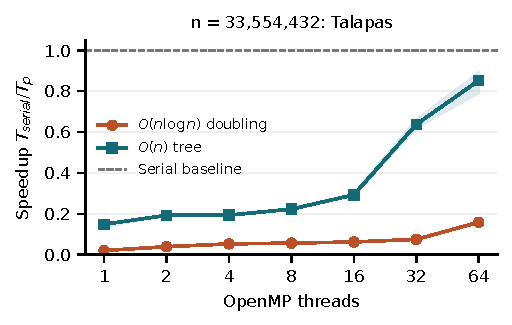
\includegraphics[width=\linewidth]{scaling.pdf}
\caption{Thread scaling at the largest input. Shading reflects runtime
IQR; the dashed line is serial performance.}
\Description{Median speedup of the doubling and tree algorithms versus thread count, with interquartile shading and a serial baseline.}
\label{fig:scaling}
\end{figure}

\FindingSummary{}
Tree traversal has strided access and barriers, while doubling performs
many full-array passes. Untimed source-copy preparation can also favor
serial cache locality. These are plausible contributors to the observed
timings; hardware-counter measurements did not isolate their effects.
\MachineLimit{}

\section*{Provenance}
Algorithms follow lecture 7, slides 43--64, and the
\href{https://github.com/UOCS431531/uoregon-cs431531-f26-assignments}{current course starter}.
The provided serial recurrence is retained, with an empty-input guard.
Code, experiment scripts, and this report were prepared with AI assistance.
The supplied course slides exclude AI coding help for homework; verify
permission before submission. Raw timings and environment records are
included with the code.
\end{document}
